We first analyze the results in terms of accuracy: how often the models correctly predicted whether a turn transition occurred or not, in other words, how often it predicts the correct value of $y_{i+1}$.
%
Table 2 shows the results of training a random forest for each model.
We see that using the summary features provides better accuracy than baseline 1, which only uses the current current dialog act ($66.14\%$ vs $60.26\%$). In addition, using the full model yields an improvement of over $1.58\%$ in the result.
%
\begin{table}[ht!]
\scriptsize
   \begin{center}
    \begin{tabular}{| l | l | l | c |}
    \hline
    Model & Accuracy & AUC & hyper parameters\\
    \hline
    Baseline 1      & 60.26\% & 0.63 & \scriptsize{max\_features=sqrt, max\_depth=7} \\
    Baseline 2     & 74.43\% & 0.79 & \scriptsize{max\_features=log2, max\_depth=9}\\
    Summary        & 66.14\% & 0.65 & \scriptsize{max\_features=sqrt, max\_depth=5} \\
    Full           & 76.05\% & 0.82 &\scriptsize{ max\_features=10, max\_depth=9}\\
  \hline
\end{tabular}
\end{center}
\vspace{-1.2em}
\caption{Accuracy and AUC results }
\end{table}

The effect can also be seen in Figure 3, which shows the ROC curves and the AUC for each
model. We notice that the AUC of the summary model is better than baseline model ($0.65$ vs $0.63$), and when adding the summary features to the local features, the full model, we see the AUC improves ($0.82$ vs $0.79$). This suggests that while the discrimination facility of the summary features is lacking (AUC $<0.7$), adding them to a classifier that uses local features (full model) yields better results than the baseline.
%
 \begin{figure}[ht!]
 \centering
 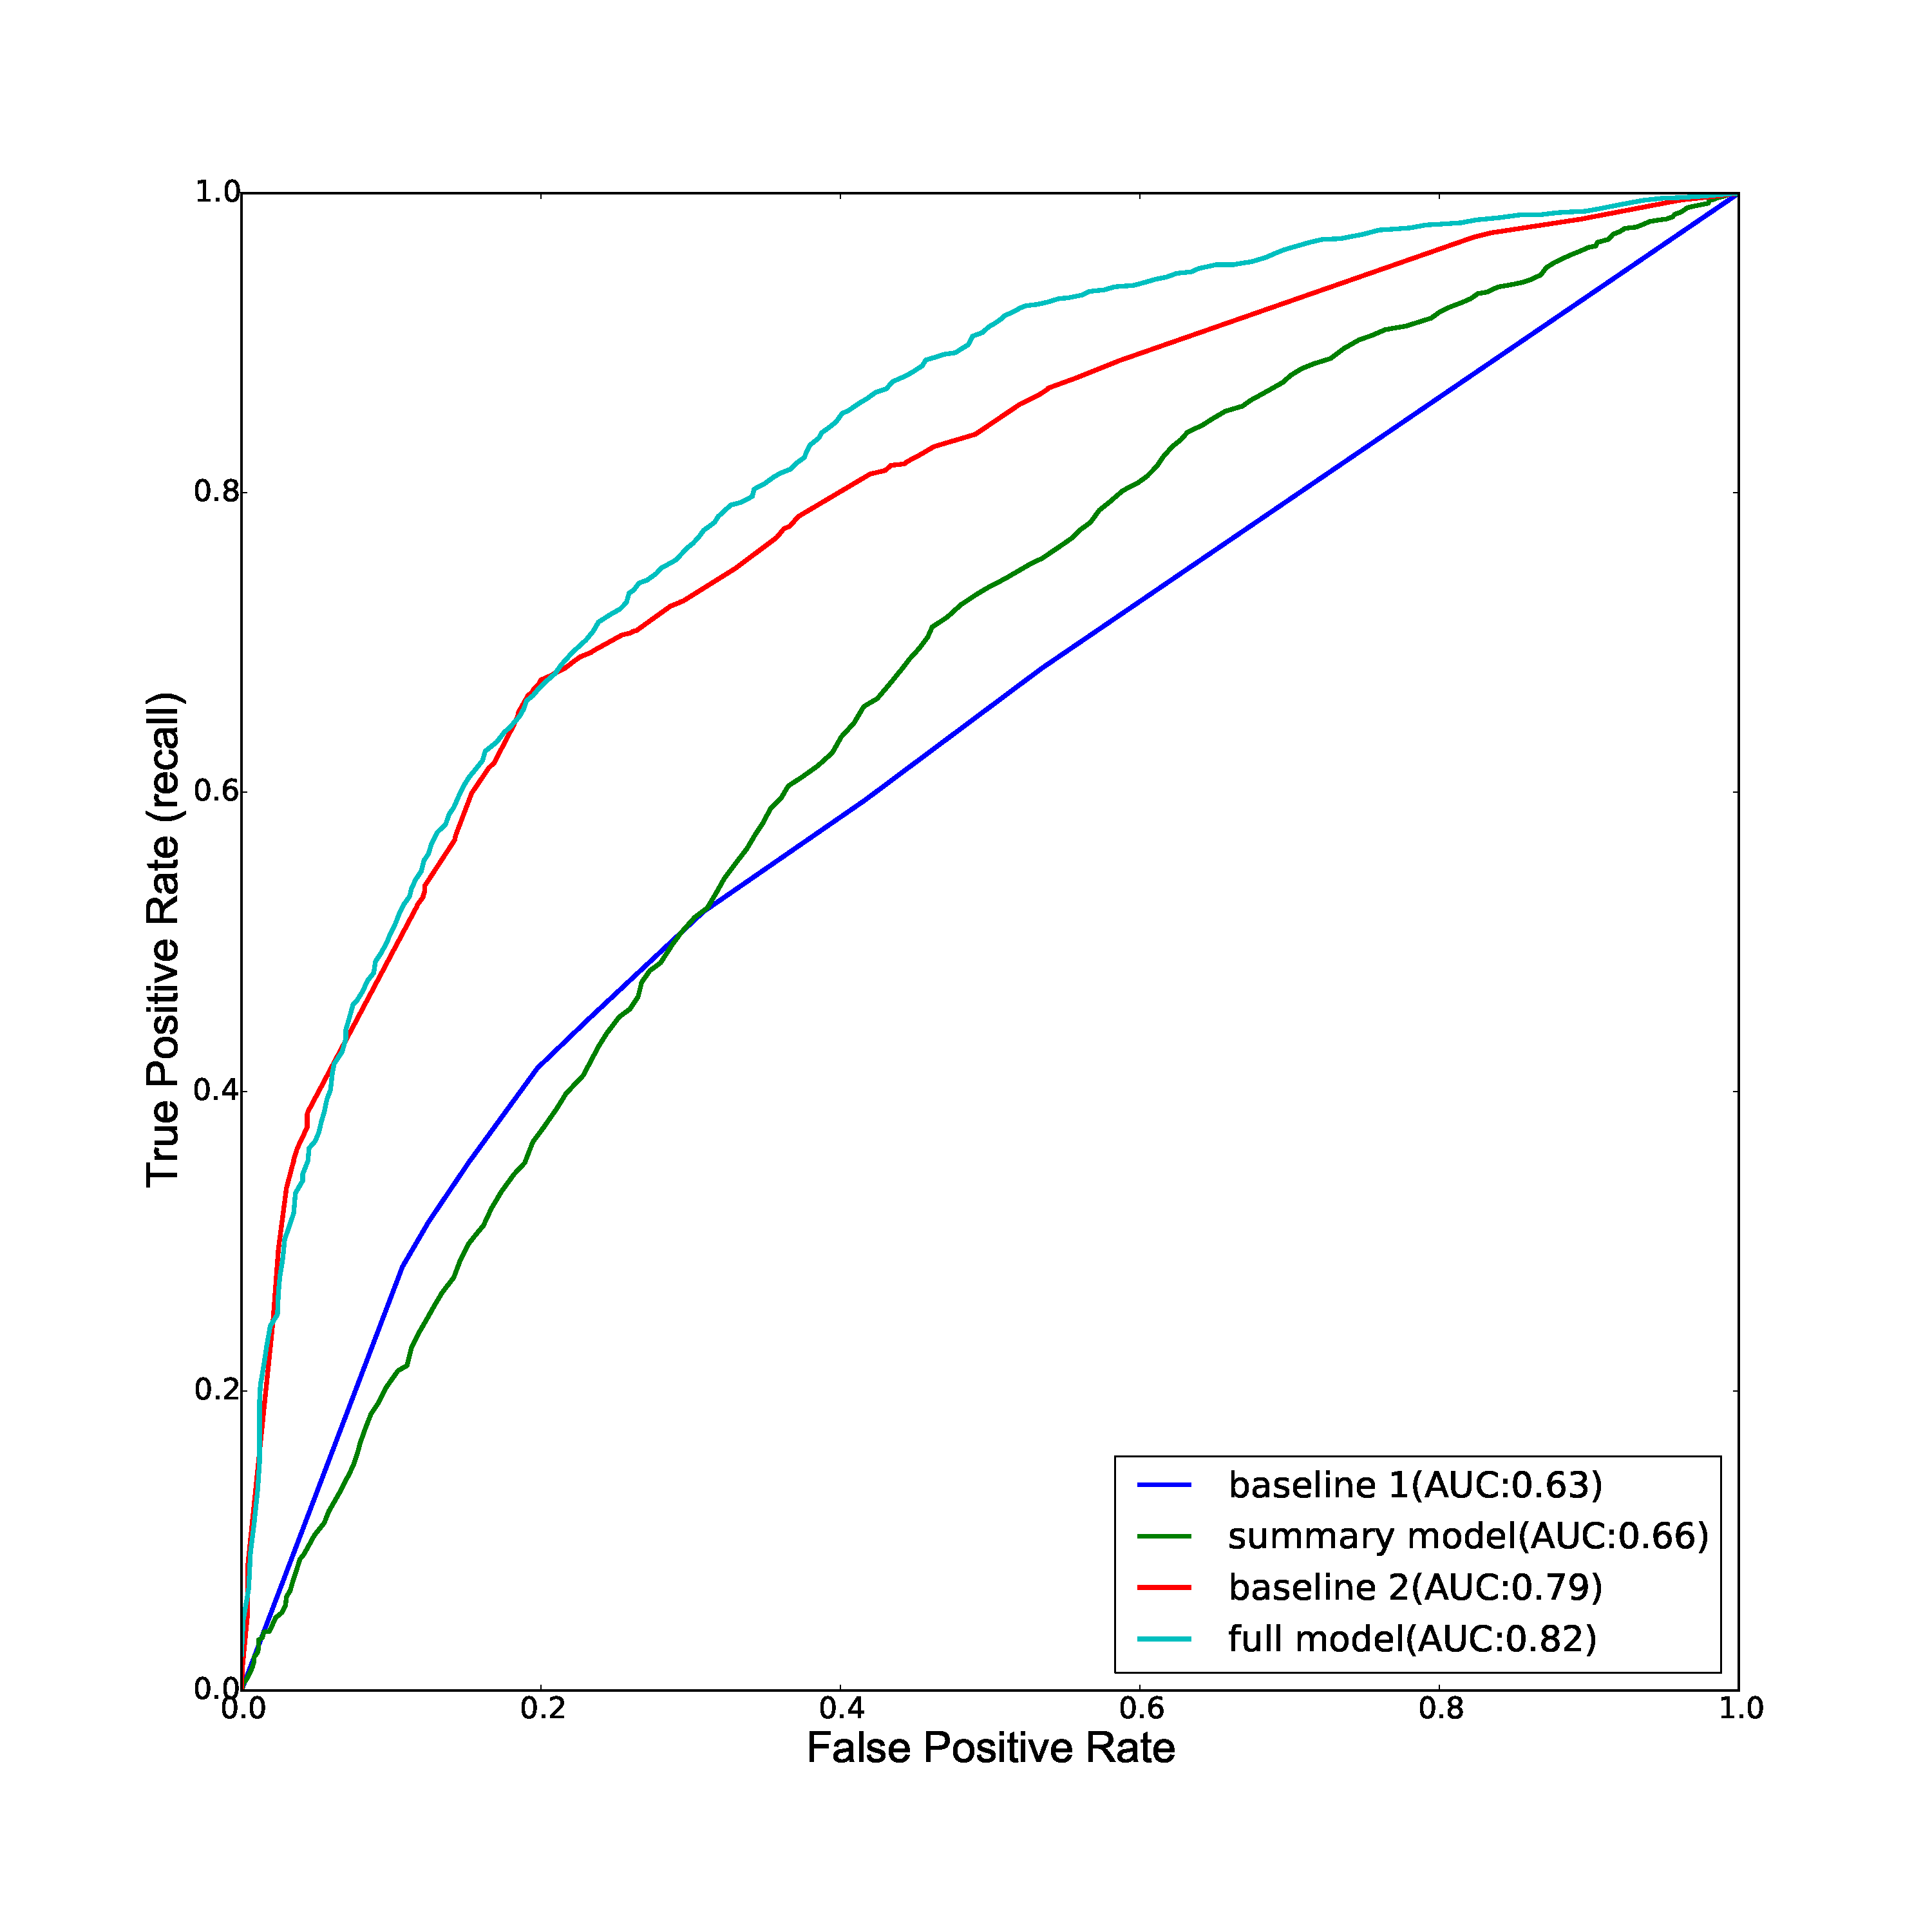
\includegraphics[width=0.5\textwidth,width=6cm,height=6cm,keepaspectratio]{roc.pdf}\vspace{-1.5em}
 \caption{ROC curves and AUC of the different models \label{overflow}}
 \end{figure}

In addition to analyzing the results in terms of accuracy, we also analyze the results of the four models in terms of how well we predict that there is a change in speaker (i.e., $y_{i+1}$  indicates that there was a turn switch).  Table 3 shows the results in terms of recall, precision, and F1, which combines the two scores.  Although baseline 1 has high precision, it has very low recall. Using only the summary model improves recall and decreases precision by less,
leading to a higher F1 score and overall better performance. Using the full model improves precision, which means that dialog acts
that were considered to lead to turn transitions are classified correctly. If we use the full model, we lose precision (over baseline 2 model), but gain recall,
leading to the highest F1 score and the best performance.
%
\begin{table}[ht!]
\scriptsize
   \begin{center}
    \begin{tabular}{|l|l|l|c|}
    \hline
    Model & Precision & Recall & F1\\
    \hline
    Baseline 1               &69.49\% &45.52\%&54.97\%\\
    Baseline 2               &80.38\% &68.80\%&74.08\%\\
    Summary                  &64.55\% &68.88\%&66.42\%\\
    Full                     &76.17\% &77.25\%&74.87\%\\
  \hline
\end{tabular}
\end{center}\vspace{-0.8em}
\caption{Precision, recall and F1 results }
\end{table}

